\documentclass{beamer}
\beamerdefaultoverlayspecification{<+->}
%
% Choose how your presentation looks.
%
% For more themes, color themes and font themes, see:
% http://deic.uab.es/~iblanes/beamer_gallery/index_by_theme.html
%
\mode<presentation>
{
  \usetheme{default}      % or try Darmstadt, Madrid, Warsaw, ...
  \usecolortheme{default} % or try albatross, beaver, crane, ...
  \usefonttheme{default}  % or try serif, structurebold, ...
  \setbeamertemplate{navigation symbols}{}
  \setbeamertemplate{caption}[numbered]
  \setbeamertemplate{footline}[frame number]
} 

\usepackage[english]{babel}
\usepackage[utf8]{inputenc}
\usepackage[T1]{fontenc}
\usepackage{graphicx}
\graphicspath{ {./images/} }
\usepackage{hyperref}
\usepackage{pgfplots}
\usepackage{float}
\pgfplotsset{compat=1.7}
\setlength{\tabcolsep}{3pt}

\hypersetup{
    colorlinks=true,
    linkcolor=blue,
    filecolor=magenta,      
    urlcolor=cyan,
    bookmarks=true,
    pdfpagemode=FullScreen,
    }

\title{Econ 200 Section AJ}
\author{Lukas Hager \\ \href{mailto:lghhager@uw.edu}{lghhager@uw.edu}}
\institute{Office Hours: Monday 8-9, Thursday 3:30-4:30}
\date{March 5, 2021}

\begin{document}

\begin{frame}
  \titlepage
\end{frame}

% Uncomment these lines for an automatically generated outline.
%\begin{frame}{Outline}
%  \tableofcontents
%\end{frame}

\begin{frame}{Your Questions}
    Do you have questions about what you've read in the text or heard in lecture?
\end{frame}

\begin{frame}{Barriers to Entry}
    \begin{itemize}
        \item What gives rise to a natural monopoly?
        \begin{itemize}
            \item A natural monopoly arises when the production function exhibits economies of scale over the relevant range of market demand. The average cost of production is lower as the output produced increases.
        \end{itemize}
        \item How do consumers benefit from a natural monopoly?
        \begin{itemize}
            \item Consumers benefit from having one supplier because the supplier will be able to pass some of the cost savings to consumers.
        \end{itemize}
    \end{itemize}
\end{frame}

\begin{frame}{Barriers to Entry}
    \begin{itemize}
        \item How does a network externality serve as a barrier to entry?
        \begin{itemize}
            \item A network externality exists where the usefulness of the product increases with the number of people who use it. It can serve as an entry barrier because the popularity of the product attracts more and more consumers, thereby increasing the supplier's dominance in the market.
        \end{itemize}
        \item Is this barrier surmountable?
        \begin{itemize}
            \item Yes. If a rival enters the market with a superior product, then it is possible that customers will switch to the superior product.
        \end{itemize}
    \end{itemize}
\end{frame}

\begin{frame}[t]{Monopoly Output}
    \begin{table}[H]
    \begin{tabular}{cccccc}
    Price/Unit & \begin{tabular}[c]{@{}c@{}}Quantity \\ Demanded\end{tabular} & \begin{tabular}[c]{@{}c@{}}Total \\ Revenue\end{tabular} & \begin{tabular}[c]{@{}c@{}}Marginal \\ Revenue\end{tabular} & \begin{tabular}[c]{@{}c@{}}Total Cost\\ of Production\end{tabular} & \begin{tabular}[c]{@{}c@{}}Marginal\\ Cost\end{tabular} \\ \hline
    85         & 10                                                           &                                                          &                                                             & 530                                                                &                                                         \\ \hline
    80         & 11                                                           &                                                          &                                                             & 540                                                                &                                                         \\ \hline
    75         & 12                                                           &                                                          &                                                             & 550                                                                &                                                         \\ \hline
    70         & 13                                                           &                                                          &                                                             & 560                                                                &                                                         \\ \hline
    65         & 14                                                           &                                                          &                                                             & 575                                                                &                                                         \\ \hline
    60         & 15                                                           &                                                          &                                                             & 595                                                                &                                                         \\ \hline
    55         & 16                                                           &                                                          &                                                             & 625                                                                &                                                        
    \end{tabular}
    \end{table}
    Complete the table.
\end{frame}

\begin{frame}[t]{Monopoly Output}
    \begin{table}[H]
    \begin{tabular}{cccccc}
    Price/Unit & \begin{tabular}[c]{@{}c@{}}Quantity \\ Demanded\end{tabular} & \begin{tabular}[c]{@{}c@{}}Total \\ Revenue\end{tabular} & \begin{tabular}[c]{@{}c@{}}Marginal \\ Revenue\end{tabular} & \begin{tabular}[c]{@{}c@{}}Total Cost\\ of Production\end{tabular} & \begin{tabular}[c]{@{}c@{}}Marginal\\ Cost\end{tabular} \\ \hline
    85         & 10                                                           & 850                                                      & --                                                          & 530                                                                & --                                                      \\ \hline
    80         & 11                                                           & 880                                                      & 30                                                          & 540                                                                & 10                                                      \\ \hline
    75         & 12                                                           & 900                                                      & 20                                                          & 550                                                                & 10                                                      \\ \hline
    70         & 13                                                           & 910                                                      & 10                                                          & 560                                                                & 10                                                      \\ \hline
    65         & 14                                                           & 910                                                      & 0                                                           & 575                                                                & 15                                                      \\ \hline
    60         & 15                                                           & 900                                                      & -10                                                         & 595                                                                & 20                                                      \\ \hline
    55         & 16                                                           & 880                                                      & -20                                                         & 625                                                                & 30                                                     
    \end{tabular}
    \end{table}
\end{frame}

\begin{frame}[t]{Monopoly Output}
    \begin{table}[H]
    \begin{tabular}{cccccc}
    Price/Unit & \begin{tabular}[c]{@{}c@{}}Quantity \\ Demanded\end{tabular} & \begin{tabular}[c]{@{}c@{}}Total \\ Revenue\end{tabular} & \begin{tabular}[c]{@{}c@{}}Marginal \\ Revenue\end{tabular} & \begin{tabular}[c]{@{}c@{}}Total Cost\\ of Production\end{tabular} & \begin{tabular}[c]{@{}c@{}}Marginal\\ Cost\end{tabular} \\ \hline
    85         & 10                                                           & 850                                                      & --                                                          & 530                                                                & --                                                      \\ \hline
    80         & 11                                                           & 880                                                      & 30                                                          & 540                                                                & 10                                                      \\ \hline
    75         & 12                                                           & 900                                                      & 20                                                          & 550                                                                & 10                                                      \\ \hline
    70         & 13                                                           & 910                                                      & 10                                                          & 560                                                                & 10                                                      \\ \hline
    65         & 14                                                           & 910                                                      & 0                                                           & 575                                                                & 15                                                      \\ \hline
    60         & 15                                                           & 900                                                      & -10                                                         & 595                                                                & 20                                                      \\ \hline
    55         & 16                                                           & 880                                                      & -20                                                         & 625                                                                & 30                                                     
    \end{tabular}
    \end{table}
    What is the monopolist's choice of output and price?
\end{frame}

\begin{frame}[t]{Monopoly Output}
    \begin{table}[H]
    \begin{tabular}{cccccc}
    Price/Unit & \begin{tabular}[c]{@{}c@{}}Quantity \\ Demanded\end{tabular} & \begin{tabular}[c]{@{}c@{}}Total \\ Revenue\end{tabular} & \begin{tabular}[c]{@{}c@{}}Marginal \\ Revenue\end{tabular} & \begin{tabular}[c]{@{}c@{}}Total Cost\\ of Production\end{tabular} & \begin{tabular}[c]{@{}c@{}}Marginal\\ Cost\end{tabular} \\ \hline
    85         & 10                                                           & 850                                                      & --                                                          & 530                                                                & --                                                      \\ \hline
    80         & 11                                                           & 880                                                      & 30                                                          & 540                                                                & 10                                                      \\ \hline
    75         & 12                                                           & 900                                                      & 20                                                          & 550                                                                & 10                                                      \\ \hline
    70         & 13                                                           & 910                                                      & 10                                                          & 560                                                                & 10                                                      \\ \hline
    65         & 14                                                           & 910                                                      & 0                                                           & 575                                                                & 15                                                      \\ \hline
    60         & 15                                                           & 900                                                      & -10                                                         & 595                                                                & 20                                                      \\ \hline
    55         & 16                                                           & 880                                                      & -20                                                         & 625                                                                & 30                                                     
    \end{tabular}
    \end{table}
    What is the monopolist’s profit?
\end{frame}

\begin{frame}[t]{Monopoly Graph}
    Find the monopolist’s output, price and profit from the diagram below:
    \newline
    \begin{center}
        \includegraphics[scale = .6]{images/monopoly_graph.png}
    \end{center}
\end{frame}

\begin{frame}[t]{Monopoly Graph}
    Find the monopolist’s output, price and profit from the diagram below: $Q = 600, P = \$34, \text{Profit} = (\$34-\$29.5) \times 600 = \$2,700$
    \newline
    \begin{center}
        \includegraphics[scale = .6]{images/monopoly_graph.png}
    \end{center}
\end{frame}

\begin{frame}{Efficiency Loss of Monopoly}
    \begin{itemize}
        \item Why does a monopoly cause a deadweight loss?
        \begin{itemize}
            \item Because it does not produce some output for which marginal benefit exceeds marginal cost.
        \end{itemize}
        \item On the figure like the one above, identify the CS and PS of the perfectly competitive outcome, then show the CS transferred to the monopolist, the PS gained by the monopolist, and the DWL.
        \item Choose the correct answer: A monopoly will produce (more/less) and charge a (higher/lower) price than would a perfectly competitive industry producing the same good.
    \end{itemize}
\end{frame}

\begin{frame}{Fast Food}
    \begin{itemize}
        \item McDonald’s, Burger King, and Wendy’s all produce hamburgers, among other things. However, if you prefer burgers from McDonald’s, you might consider other burgers an imperfect substitute. With this in mind, how would you expect McDonald’s to set its prices in the short run? Describe the relationship between price, marginal revenue, and marginal cost.
        \begin{itemize}
            \item In the short run, McDonald’s will set its prices like a monopolist. McDonald’s will maximize profits by producing where marginal revenue equals marginal cost and charging the highest price that demand will bear. If this price happens to be more than Burger King and Wendy’s, consumers will pay the price differential as long as it is not greater than the value they place on their preference for McDonald’s burgers over its competitors.
        \end{itemize}
    \end{itemize}
\end{frame}

\begin{frame}{Jimmy Choo}
    \begin{itemize}
        \item Consider Jimmy Choo designer shoes. In what way does Jimmy Choo face many competitors? In what way does Jimmy Choo face no competitors?
        \begin{itemize}
            \item Jimmy Choo is a small player in the market for shoes and faces many competitors. However, Jimmy Choo is a monopolist for Jimmy Choo designer shoes. How much Jimmy Choo can charge for shoes bearing its label will depend on how substitutable consumers think other shoes are as a substitute for Jimmy Choo shoes.
        \end{itemize}
    \end{itemize}
\end{frame}

\begin{frame}{Restaurants}
    \begin{itemize}
        \item Restaurants offer related but differentiated products to their consumers. In the long run, new restaurants enter the market and imitate the cuisine and atmosphere of successful competitors. How would you expect a restaurant to set its prices in the long run? Describe the relationship between price and average total cost. Does a restaurant earn economic profits?
        \begin{itemize}
            \item In the long run, restaurants will enter the market as long as there are positive profits. As more competitors and substitutes enter, the demand curve for a particular restaurant will shift to the left. This will continue until there are no longer economic profits. Price will be equal to ATC in the long run for firms in a monopolistically competitive market.
        \end{itemize}
    \end{itemize}
\end{frame}

\begin{frame}[t]{Smartphones}
    \begin{center}
        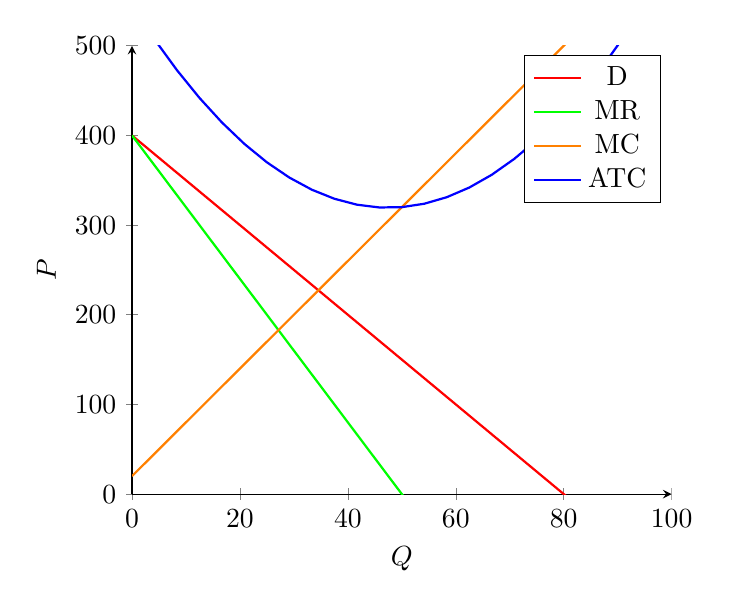
\begin{tikzpicture}
        \begin{axis}[
            axis lines = left,
            xlabel = $Q$,
            ylabel = $P$,
            ymax = 500,
            ymin = 0,
            xmax = 100,
            xmin = 0,
            scaled x ticks = false
            % ytick = {0,1,1.5,2,3,5},
            % xtick = {0,3,6,12,18,21}
        ]
        \addplot[
        color=red,thick,
        domain=0:500,
        range = 0:500]{-5*x + 400};
        \addlegendentry{D}
        \addplot[
        color=green,thick,
        domain=0:500,
        range = 0:500]{-8*x + 400};
        \addlegendentry{MR}
        \addplot[
        color=orange,thick,
        domain=0:500,
        range = 0:500]{6*x + 20};
        \addlegendentry{MC}
        \addplot[
        color=blue,thick,
        domain=0:100,
        range = 0:50]{(x-50)^2/10 + .5*(x-50) + 320};
        \addlegendentry{ATC}
        % \addplot[
        % color=blue,thick,dashed,
        % domain=0:50,
        % range = 0:50]{1.5};
        % \addlegendentry{{World Price ($P_W$)}}
        % \addplot[
        % color=blue,thick,dotted,
        % domain=0:50,
        % range = 0:50]{2};
        % \addlegendentry{{$P_W$ + Tariff}}
        % \addplot[
        % black,thick,dashed]
        % coordinates {
        %     (12,0)
        %     (12,3)
        %     (0,3)
        % };
        % \addplot[
        % black,thick,dashed]
        % coordinates {
        %     (3,1.5)
        %     (3,0)
        % };
        % \addplot[
        % black,thick,dashed]
        % coordinates {
        %     (21,1.5)
        %     (21,0)
        % };
        % \addplot[
        % black,thick,dashed]
        % coordinates {
        %     (6,2)
        %     (6,0)
        % };
        % \addplot[
        % black,thick,dashed]
        % coordinates {
        %     (18,2)
        %     (18,0)
        % };
        \end{axis}
        \end{tikzpicture}
    \end{center}
    Plot the profit-maximizing price and quantity on the graph. Is this producer earning positive or negative profits in the short run?
\end{frame}

\begin{frame}[t]{Smartphones}
    \begin{center}
        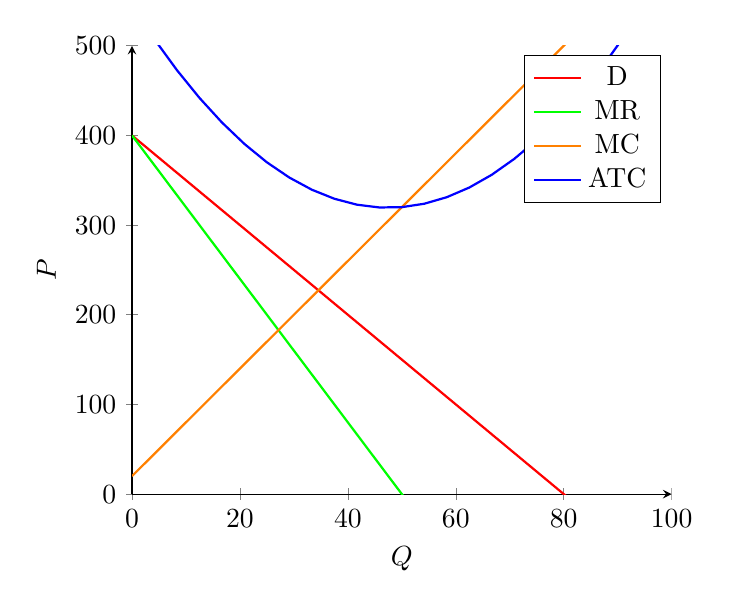
\begin{tikzpicture}
        \begin{axis}[
            axis lines = left,
            xlabel = $Q$,
            ylabel = $P$,
            ymax = 500,
            ymin = 0,
            xmax = 100,
            xmin = 0,
            scaled x ticks = false
            % ytick = {0,1,1.5,2,3,5},
            % xtick = {0,3,6,12,18,21}
        ]
        \addplot[
        color=red,thick,
        domain=0:500,
        range = 0:500]{-5*x + 400};
        \addlegendentry{D}
        \addplot[
        color=green,thick,
        domain=0:500,
        range = 0:500]{-8*x + 400};
        \addlegendentry{MR}
        \addplot[
        color=orange,thick,
        domain=0:500,
        range = 0:500]{6*x + 20};
        \addlegendentry{MC}
        \addplot[
        color=blue,thick,
        domain=0:100,
        range = 0:50]{(x-50)^2/10 + .5*(x-50) + 320};
        \addlegendentry{ATC}
        % \addplot[
        % color=blue,thick,dashed,
        % domain=0:50,
        % range = 0:50]{1.5};
        % \addlegendentry{{World Price ($P_W$)}}
        % \addplot[
        % color=blue,thick,dotted,
        % domain=0:50,
        % range = 0:50]{2};
        % \addlegendentry{{$P_W$ + Tariff}}
        % \addplot[
        % black,thick,dashed]
        % coordinates {
        %     (12,0)
        %     (12,3)
        %     (0,3)
        % };
        % \addplot[
        % black,thick,dashed]
        % coordinates {
        %     (3,1.5)
        %     (3,0)
        % };
        % \addplot[
        % black,thick,dashed]
        % coordinates {
        %     (21,1.5)
        %     (21,0)
        % };
        % \addplot[
        % black,thick,dashed]
        % coordinates {
        %     (6,2)
        %     (6,0)
        % };
        % \addplot[
        % black,thick,dashed]
        % coordinates {
        %     (18,2)
        %     (18,0)
        % };
        \end{axis}
        \end{tikzpicture}
    \end{center}
    In the long run, will supply or demand for this producer's good be affected? Will economic profits increase or decrease?
\end{frame}

\begin{frame}{SqueakyKleen}
    \begin{center}
        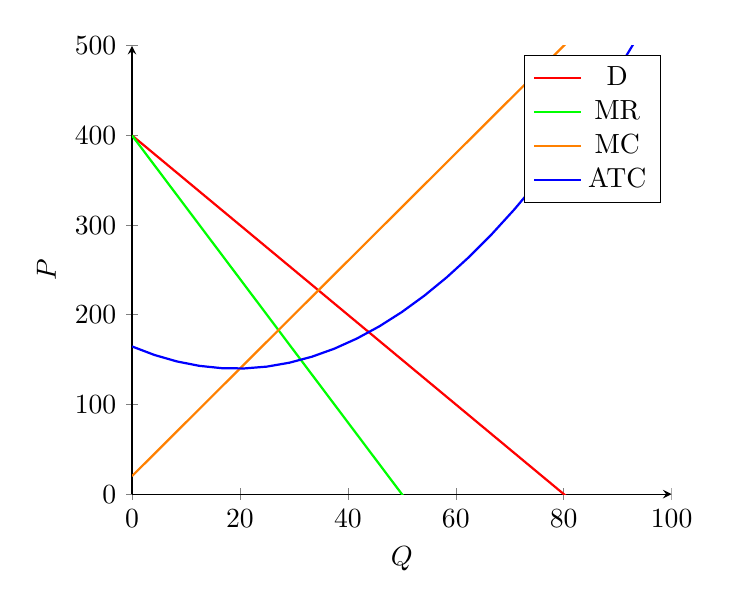
\begin{tikzpicture}
        \begin{axis}[
            axis lines = left,
            xlabel = $Q$,
            ylabel = $P$,
            ymax = 500,
            ymin = 0,
            xmax = 100,
            xmin = 0,
            scaled x ticks = false
            % ytick = {0,1,1.5,2,3,5},
            % xtick = {0,3,6,12,18,21}
        ]
        \addplot[
        color=red,thick,
        domain=0:500,
        range = 0:500]{-5*x + 400};
        \addlegendentry{D}
        \addplot[
        color=green,thick,
        domain=0:500,
        range = 0:500]{-8*x + 400};
        \addlegendentry{MR}
        \addplot[
        color=orange,thick,
        domain=0:500,
        range = 0:500]{6*x + 20};
        \addlegendentry{MC}
        \addplot[
        color=blue,thick,
        domain=0:100,
        range = 0:50]{(x-20)^2/15 + .1 * (x-20) + 140};
        \addlegendentry{ATC}
        % \addplot[
        % color=blue,thick,dashed,
        % domain=0:50,
        % range = 0:50]{1.5};
        % \addlegendentry{{World Price ($P_W$)}}
        % \addplot[
        % color=blue,thick,dotted,
        % domain=0:50,
        % range = 0:50]{2};
        % \addlegendentry{{$P_W$ + Tariff}}
        % \addplot[
        % black,thick,dashed]
        % coordinates {
        %     (12,0)
        %     (12,3)
        %     (0,3)
        % };
        % \addplot[
        % black,thick,dashed]
        % coordinates {
        %     (3,1.5)
        %     (3,0)
        % };
        % \addplot[
        % black,thick,dashed]
        % coordinates {
        %     (21,1.5)
        %     (21,0)
        % };
        % \addplot[
        % black,thick,dashed]
        % coordinates {
        %     (6,2)
        %     (6,0)
        % };
        % \addplot[
        % black,thick,dashed]
        % coordinates {
        %     (18,2)
        %     (18,0)
        % };
        \end{axis}
        \end{tikzpicture}
    \end{center}
    What is the price and quantity of SqueakyKleen, a monopolistically competitive firm, in the short run?
\end{frame}

\begin{frame}{SqueakyKleen}
    \begin{center}
        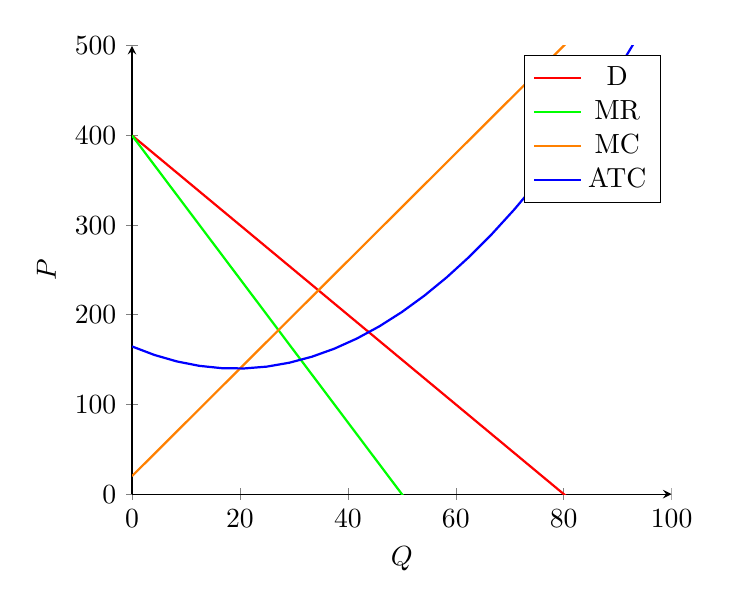
\begin{tikzpicture}
        \begin{axis}[
            axis lines = left,
            xlabel = $Q$,
            ylabel = $P$,
            ymax = 500,
            ymin = 0,
            xmax = 100,
            xmin = 0,
            scaled x ticks = false
            % ytick = {0,1,1.5,2,3,5},
            % xtick = {0,3,6,12,18,21}
        ]
        \addplot[
        color=red,thick,
        domain=0:500,
        range = 0:500]{-5*x + 400};
        \addlegendentry{D}
        \addplot[
        color=green,thick,
        domain=0:500,
        range = 0:500]{-8*x + 400};
        \addlegendentry{MR}
        \addplot[
        color=orange,thick,
        domain=0:500,
        range = 0:500]{6*x + 20};
        \addlegendentry{MC}
        \addplot[
        color=blue,thick,
        domain=0:100,
        range = 0:50]{(x-20)^2/15 + .1 * (x-20) + 140};
        \addlegendentry{ATC}
        % \addplot[
        % color=blue,thick,dashed,
        % domain=0:50,
        % range = 0:50]{1.5};
        % \addlegendentry{{World Price ($P_W$)}}
        % \addplot[
        % color=blue,thick,dotted,
        % domain=0:50,
        % range = 0:50]{2};
        % \addlegendentry{{$P_W$ + Tariff}}
        % \addplot[
        % black,thick,dashed]
        % coordinates {
        %     (12,0)
        %     (12,3)
        %     (0,3)
        % };
        % \addplot[
        % black,thick,dashed]
        % coordinates {
        %     (3,1.5)
        %     (3,0)
        % };
        % \addplot[
        % black,thick,dashed]
        % coordinates {
        %     (21,1.5)
        %     (21,0)
        % };
        % \addplot[
        % black,thick,dashed]
        % coordinates {
        %     (6,2)
        %     (6,0)
        % };
        % \addplot[
        % black,thick,dashed]
        % coordinates {
        %     (18,2)
        %     (18,0)
        % };
        \end{axis}
        \end{tikzpicture}
    \end{center}
    What is the efficient price and quantity of SqueakyKleen?
\end{frame}

\begin{frame}{SqueakyKleen}
    \begin{center}
        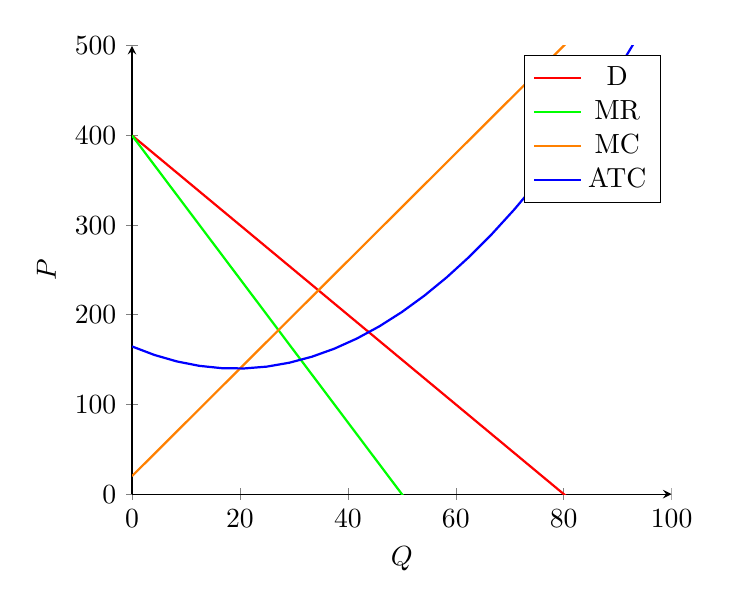
\begin{tikzpicture}
        \begin{axis}[
            axis lines = left,
            xlabel = $Q$,
            ylabel = $P$,
            ymax = 500,
            ymin = 0,
            xmax = 100,
            xmin = 0,
            scaled x ticks = false
            % ytick = {0,1,1.5,2,3,5},
            % xtick = {0,3,6,12,18,21}
        ]
        \addplot[
        color=red,thick,
        domain=0:500,
        range = 0:500]{-5*x + 400};
        \addlegendentry{D}
        \addplot[
        color=green,thick,
        domain=0:500,
        range = 0:500]{-8*x + 400};
        \addlegendentry{MR}
        \addplot[
        color=orange,thick,
        domain=0:500,
        range = 0:500]{6*x + 20};
        \addlegendentry{MC}
        \addplot[
        color=blue,thick,
        domain=0:100,
        range = 0:50]{(x-20)^2/15 + .1 * (x-20) + 140};
        \addlegendentry{ATC}
        % \addplot[
        % color=blue,thick,dashed,
        % domain=0:50,
        % range = 0:50]{1.5};
        % \addlegendentry{{World Price ($P_W$)}}
        % \addplot[
        % color=blue,thick,dotted,
        % domain=0:50,
        % range = 0:50]{2};
        % \addlegendentry{{$P_W$ + Tariff}}
        % \addplot[
        % black,thick,dashed]
        % coordinates {
        %     (12,0)
        %     (12,3)
        %     (0,3)
        % };
        % \addplot[
        % black,thick,dashed]
        % coordinates {
        %     (3,1.5)
        %     (3,0)
        % };
        % \addplot[
        % black,thick,dashed]
        % coordinates {
        %     (21,1.5)
        %     (21,0)
        % };
        % \addplot[
        % black,thick,dashed]
        % coordinates {
        %     (6,2)
        %     (6,0)
        % };
        % \addplot[
        % black,thick,dashed]
        % coordinates {
        %     (18,2)
        %     (18,0)
        % };
        \end{axis}
        \end{tikzpicture}
    \end{center}
    Draw the deadweight loss.
\end{frame}

\begin{frame}{A Challenge For My Graphing Skills}
    \begin{center}
        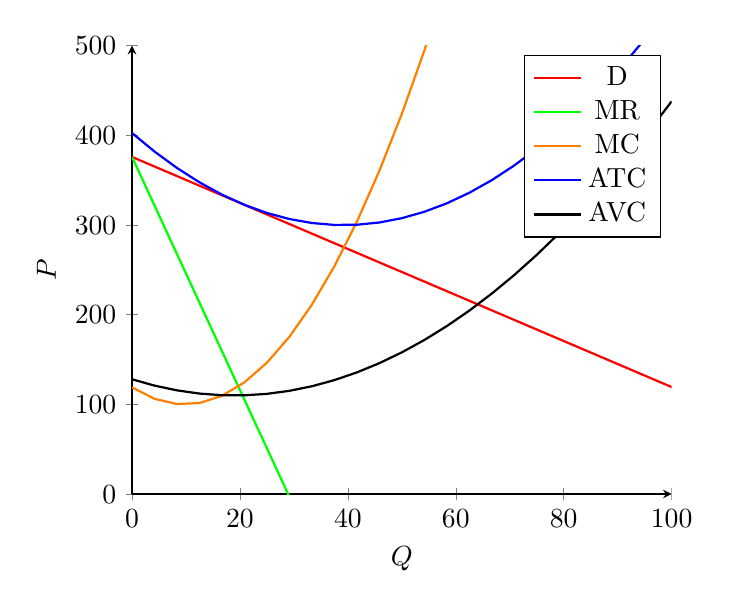
\begin{tikzpicture}
        \begin{axis}[
            axis lines = left,
            xlabel = $Q$,
            ylabel = $P$,
            ymax = 500,
            ymin = 0,
            xmax = 100,
            xmin = 0,
            scaled x ticks = false
            % ytick = {0,1,1.5,2,3,5},
            % xtick = {0,3,6,12,18,21}
        ]
        \addplot[
        color=red,thick,
        domain=0:500,
        range = 0:500]{376 - 2.56667*x};
        \addlegendentry{D}
        \addplot[
        color=green,thick,
        domain=0:500,
        range = 0:500]{376 - 13*x};
        \addlegendentry{MR}
        \addplot[
        color=orange,thick,
        domain=0:100,
        range = 0:50]{(x-10)^2/5 + .1 * (x-10) + 100};
        \addlegendentry{MC}
        \addplot[
        color=blue,thick,
        domain=0:100,
        range = 0:50]{(x-40)^2/15 + .1 * (x-40) + 300};
        \addlegendentry{ATC}
        \addplot[
        color=black,thick,
        domain=0:100,
        range = 0:50]{(x-20)^2/20 + .1 * (x-20) + 110};
        \addlegendentry{AVC}
        % \addplot[
        % color=blue,thick,dashed,
        % domain=0:50,
        % range = 0:50]{1.5};
        % \addlegendentry{{World Price ($P_W$)}}
        % \addplot[
        % color=blue,thick,dotted,
        % domain=0:50,
        % range = 0:50]{2};
        % \addlegendentry{{$P_W$ + Tariff}}
        % \addplot[
        % black,thick,dashed]
        % coordinates {
        %     (12,0)
        %     (12,3)
        %     (0,3)
        % };
        % \addplot[
        % black,thick,dashed]
        % coordinates {
        %     (3,1.5)
        %     (3,0)
        % };
        % \addplot[
        % black,thick,dashed]
        % coordinates {
        %     (21,1.5)
        %     (21,0)
        % };
        % \addplot[
        % black,thick,dashed]
        % coordinates {
        %     (6,2)
        %     (6,0)
        % };
        % \addplot[
        % black,thick,dashed]
        % coordinates {
        %     (18,2)
        %     (18,0)
        % };
        \end{axis}
        \end{tikzpicture}
    \end{center}
    For this monopolistically competitive firm, plot the profit-maximizing price and quantity on the graph.
\end{frame}

\begin{frame}{A Challenge For My Graphing Skills}
    \begin{center}
        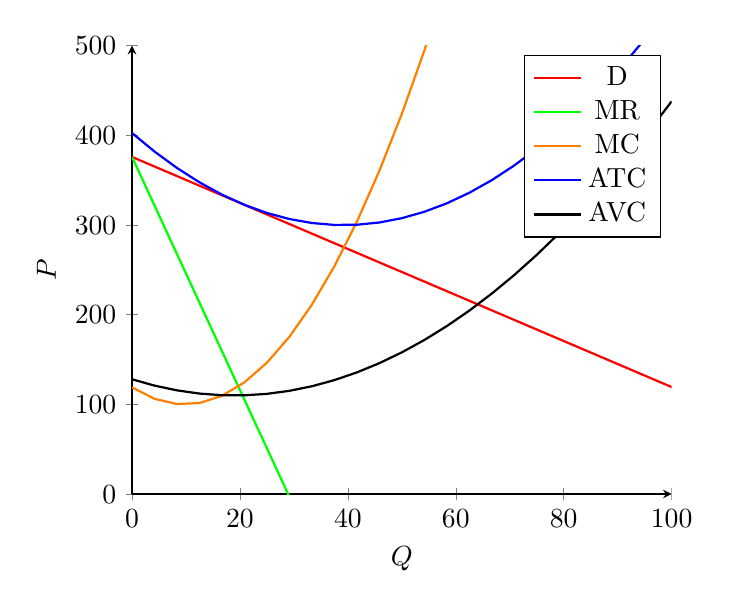
\begin{tikzpicture}
        \begin{axis}[
            axis lines = left,
            xlabel = $Q$,
            ylabel = $P$,
            ymax = 500,
            ymin = 0,
            xmax = 100,
            xmin = 0,
            scaled x ticks = false
            % ytick = {0,1,1.5,2,3,5},
            % xtick = {0,3,6,12,18,21}
        ]
        \addplot[
        color=red,thick,
        domain=0:500,
        range = 0:500]{376 - 2.56667*x};
        \addlegendentry{D}
        \addplot[
        color=green,thick,
        domain=0:500,
        range = 0:500]{376 - 13*x};
        \addlegendentry{MR}
        \addplot[
        color=orange,thick,
        domain=0:100,
        range = 0:50]{(x-10)^2/5 + .1 * (x-10) + 100};
        \addlegendentry{MC}
        \addplot[
        color=blue,thick,
        domain=0:100,
        range = 0:50]{(x-40)^2/15 + .1 * (x-40) + 300};
        \addlegendentry{ATC}
        \addplot[
        color=black,thick,
        domain=0:100,
        range = 0:50]{(x-20)^2/20 + .1 * (x-20) + 110};
        \addlegendentry{AVC}
        % \addplot[
        % color=blue,thick,dashed,
        % domain=0:50,
        % range = 0:50]{1.5};
        % \addlegendentry{{World Price ($P_W$)}}
        % \addplot[
        % color=blue,thick,dotted,
        % domain=0:50,
        % range = 0:50]{2};
        % \addlegendentry{{$P_W$ + Tariff}}
        % \addplot[
        % black,thick,dashed]
        % coordinates {
        %     (12,0)
        %     (12,3)
        %     (0,3)
        % };
        % \addplot[
        % black,thick,dashed]
        % coordinates {
        %     (3,1.5)
        %     (3,0)
        % };
        % \addplot[
        % black,thick,dashed]
        % coordinates {
        %     (21,1.5)
        %     (21,0)
        % };
        % \addplot[
        % black,thick,dashed]
        % coordinates {
        %     (6,2)
        %     (6,0)
        % };
        % \addplot[
        % black,thick,dashed]
        % coordinates {
        %     (18,2)
        %     (18,0)
        % };
        \end{axis}
        \end{tikzpicture}
    \end{center}
    Is this firm earning zero, positive, or negative profits? Why?
\end{frame}

\begin{frame}{A Challenge For My Graphing Skills}
    \begin{center}
        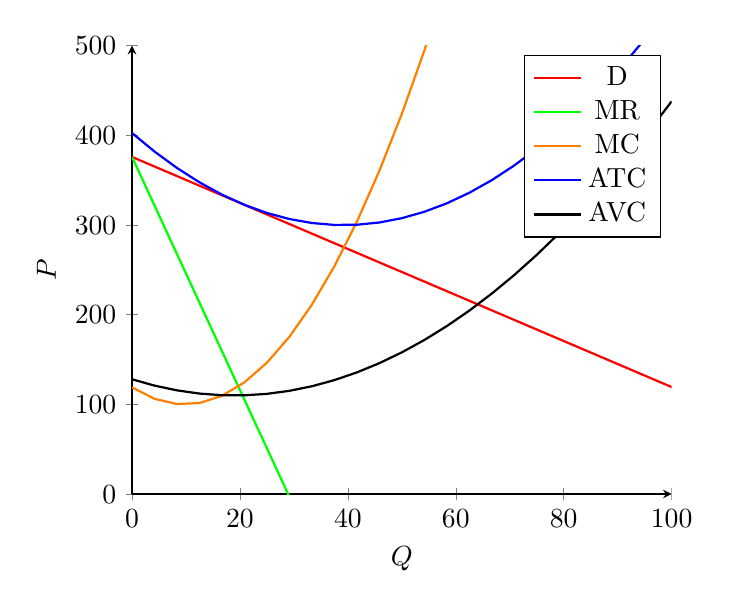
\begin{tikzpicture}
        \begin{axis}[
            axis lines = left,
            xlabel = $Q$,
            ylabel = $P$,
            ymax = 500,
            ymin = 0,
            xmax = 100,
            xmin = 0,
            scaled x ticks = false
            % ytick = {0,1,1.5,2,3,5},
            % xtick = {0,3,6,12,18,21}
        ]
        \addplot[
        color=red,thick,
        domain=0:500,
        range = 0:500]{376 - 2.56667*x};
        \addlegendentry{D}
        \addplot[
        color=green,thick,
        domain=0:500,
        range = 0:500]{376 - 13*x};
        \addlegendentry{MR}
        \addplot[
        color=orange,thick,
        domain=0:100,
        range = 0:50]{(x-10)^2/5 + .1 * (x-10) + 100};
        \addlegendentry{MC}
        \addplot[
        color=blue,thick,
        domain=0:100,
        range = 0:50]{(x-40)^2/15 + .1 * (x-40) + 300};
        \addlegendentry{ATC}
        \addplot[
        color=black,thick,
        domain=0:100,
        range = 0:50]{(x-20)^2/20 + .1 * (x-20) + 110};
        \addlegendentry{AVC}
        % \addplot[
        % color=blue,thick,dashed,
        % domain=0:50,
        % range = 0:50]{1.5};
        % \addlegendentry{{World Price ($P_W$)}}
        % \addplot[
        % color=blue,thick,dotted,
        % domain=0:50,
        % range = 0:50]{2};
        % \addlegendentry{{$P_W$ + Tariff}}
        % \addplot[
        % black,thick,dashed]
        % coordinates {
        %     (12,0)
        %     (12,3)
        %     (0,3)
        % };
        % \addplot[
        % black,thick,dashed]
        % coordinates {
        %     (3,1.5)
        %     (3,0)
        % };
        % \addplot[
        % black,thick,dashed]
        % coordinates {
        %     (21,1.5)
        %     (21,0)
        % };
        % \addplot[
        % black,thick,dashed]
        % coordinates {
        %     (6,2)
        %     (6,0)
        % };
        % \addplot[
        % black,thick,dashed]
        % coordinates {
        %     (18,2)
        %     (18,0)
        % };
        \end{axis}
        \end{tikzpicture}
    \end{center}
    Is this firm in a long-run equilibrium?
\end{frame}

\begin{frame}{Helpful Chart}
    \includegraphics[scale = .3]{images/Screen Shot 2021-03-05 at 8.50.14 AM.png}
\end{frame}

\end{document}
